\documentclass{scrartcl}
\usepackage{graphicx}

% for cyrillic and Bulgarian language
\usepackage[utf8]{inputenc}
\usepackage[T2A]{fontenc}
\usepackage[bulgarian]{babel}

% math packages
\usepackage{amsmath}
\usepackage{float}
\usepackage{amsfonts}
\usepackage{amssymb}
\usepackage{amsthm}
\usepackage{cancel}

\usepackage{ragged2e}
\usepackage{enumitem}
\usepackage{array}
\usepackage{longtable}
\usepackage{tikz}
\usetikzlibrary{arrows.meta, positioning, shapes.geometric}

\usepackage[colorlinks=true, linkcolor=blue, urlcolor=cyan]{hyperref}

\title{Управление на проекти}
\author{Ивайло Андреев + chat gpt 5.5}
\date{27 май 2026}

\begin{document}

\maketitle

\tableofcontents

\newpage

\begin{FlushLeft}

\section{Планиране на проекта – същност и основни елементи}

\subsection{Същност на планирането на проекта}

Проектът представлява временно начинание, насочено към създаване на конкретен продукт, услуга или резултат. Всеки проект има ясно определени цели, ограничени ресурси, фиксирани срокове и критерии за качество.

Основните характеристики на проекта са:

\begin{itemize}
    \item \textbf{Временност (temporality)} – проектът има начало и край;
    \item \textbf{Уникалност на резултата (deliverables)} – създава се нов продукт, услуга или знание;
    \item \textbf{Прогресивно развитие (progressive elaboration)} – проектът се уточнява и развива постепенно;
    \item \textbf{Ограниченост на ресурсите} – налични са ограничения във време, бюджет и персонал;
    \item \textbf{Наличие на риск} – съществуват несигурности и възможни проблеми при изпълнението.
\end{itemize}

Планирането на проекта е процес на определяне на необходимите дейности, ресурси, срокове, бюджет и механизми за контрол, чрез които проектът да бъде успешно реализиран.

Основната цел на планирането е:

\begin{itemize}
    \item да се дефинират целите на проекта;
    \item да се разпредели работата между участниците;
    \item да се определят сроковете и ресурсите;
    \item да се минимизират рисковете;
    \item да се осигури контрол върху изпълнението.
\end{itemize}

\subsection{Основни елементи на плана на проекта}

Планът на проекта определя как проектът ще бъде изпълняван, наблюдаван, контролиран и приключен.

Той включва набор от взаимосвързани подпланове:

\begin{itemize}
    \item \textbf{Обхват (Scope)} – определя какво влиза и какво не влиза в проекта;
    \item \textbf{График (Schedule)} – определя последователността и времето за изпълнение на задачите;
    \item \textbf{Разходи (Cost)} – определя бюджета и финансовите ограничения;
    \item \textbf{Качество (Quality)} – задава критерии за качество и контрол;
    \item \textbf{Човешки ресурси (Staffing)} – определя необходимите специалисти и роли;
    \item \textbf{Комуникации (Communication)} – дефинира обмена на информация;
    \item \textbf{Риск (Risk)} – описва възможните рискове и стратегии за реакция;
    \item \textbf{Доставки и поръчки (Procurement)} – управление на външни изпълнители и доставки;
    \item \textbf{Управление на процесите} – координация и оптимизация на проектните дейности.
\end{itemize}

\subsection{Методи и средства, използвани при планирането}

При планирането на проекта се използват различни методи и инструменти:

\begin{itemize}
    \item \textbf{Експертни оценки} – използване на знанията и опита на специалисти за оценка на задачи, рискове и ресурси;
    \item \textbf{Интервюта и анкети} – директно събиране на информация от заинтересованите страни (stakeholders) за техните нужди и очаквания;
    \item \textbf{Brainstorming} – групова техника за генериране на идеи и решения без критика в началния етап;
    \item \textbf{Анализ на риска} – идентифициране, оценяване и приоритизиране на потенциални заплахи за успешното изпълнение на проекта;
    \item \textbf{Work Breakdown Structure (WBS)} – йерархично разбиване на проекта на по-малки, управляеми работни пакети;
    \item \textbf{GANTT диаграми} – визуално представяне на задачите по времева ос с показване на продължителността и зависимостите;
    \item \textbf{PERT и CPM методи} – техники за оценка на времетраенето на задачите и определяне на критичния път в проекта;
    \item \textbf{Специализиран софтуер} – инструменти като Microsoft Project, Jira, Trello и Asana за автоматизиране на планирането и проследяването.
\end{itemize}

\section{Планиране на обхвата на проекта}

\subsection{Същност на обхвата}

Обхватът определя каква работа трябва да бъде извършена, за да се постигнат целите на проекта.

Разграничават се два основни типа обхват:

\begin{itemize}
    \item \textbf{Обхват на продукта} – функционалности и характеристики на крайния продукт;
    \item \textbf{Обхват на проекта} – всички дейности, необходими за създаването на продукта.
\end{itemize}

Неправилно дефинираният обхват е една от основните причини за провал на проекти, тъй като води до:

\begin{itemize}
    \item увеличаване на разходите;
    \item забавяне на сроковете;
    \item неясни изисквания;
    \item конфликти между участниците.
\end{itemize}

\subsection{Процеси при управление на обхвата}

Управлението на обхвата включва следните основни процеси:

\begin{enumerate}
    \item Планиране на управлението на обхвата;
    \item Събиране на изисквания;
    \item Дефиниране на обхвата;
    \item Създаване на WBS структура;
    \item Верифициране на обхвата;
    \item Контрол на промените в обхвата.
\end{enumerate}

\subsection{Събиране на изисквания}

Събирането на изисквания е процес на определяне и документиране на нуждите на заинтересованите страни.

Основни техники:

\begin{itemize}
    \item \textbf{Интервюта} – директни разговори с клиенти и заинтересовани страни за изясняване на нуждите и очакванията им;
    \item \textbf{Фокус групи} – дискусии с представители на различни потребителски групи за събиране на разнообразни гледни точки;
    \item \textbf{Workshops} – съвместни работни сесии, в които участниците дефинират и приоритизират изискванията заедно;
    \item \textbf{Анкети и въпросници} – структурирано събиране на информация от голям брой участници, когато директен контакт е невъзможен;
    \item \textbf{Наблюдение} – пряко наблюдение на работния процес за разкриване на неявни изисквания, които потребителите не могат да изразят вербално;
    \item \textbf{Прототипиране} – създаване на ранен модел на продукта за валидиране на изискванията с потребителите преди пълна реализация;
    \item \textbf{Групови техники за вземане на решения} – методи като гласуване и консенсус за приоритизиране на конкуриращи се изисквания.
\end{itemize}

Изходът от процеса включва:

\begin{itemize}
    \item документация на изискванията;
    \item матрица за проследяване на изискванията;
    \item план за управление на изискванията.
\end{itemize}

\subsection{Определяне на структура на работа (WBS)}

Йерархичната структура на работата (Work Breakdown Structure – WBS) представлява процес на разделяне на проекта на по-малки и по-лесно управляеми компоненти.

Основната идея на WBS е сложният проект да бъде декомпозиран на работни пакети.

Стъпки при изграждане на WBS:

\begin{enumerate}
    \item Определяне на основните резултати от проекта;
    \item Разделяне на резултатите на подзадачи;
    \item Детайлизиране на дейностите;
    \item Определяне на работни пакети;
    \item Проверка за пълнота и логическа свързаност.
\end{enumerate}

Всеки работен пакет включва:

\begin{itemize}
    \item описание на дейността;
    \item отговорен екип или изпълнител;
    \item необходими ресурси;
    \item срок за изпълнение;
    \item критерии за приемане;
    \item зависимости от други задачи.
\end{itemize}

\subsection{План на контролните точки}

Контролните точки (milestones) са важни събития в жизнения цикъл на проекта.

Те:

\begin{itemize}
    \item маркират завършването на ключови фази;
    \item позволяват проследяване на напредъка;
    \item улесняват комуникацията между участниците;
    \item служат като средство за контрол.
\end{itemize}

Видове контролни точки:

\begin{enumerate}
    \item \textbf{Основни контролни точки} – маркират завършването на ключови фази на проекта и обикновено изискват официално одобрение от ръководството или клиента;
    \item \textbf{Второстепенни контролни точки} – вътрешни за екипа точки за проследяване на напредъка в рамките на отделна фаза;
    \item \textbf{Контролни точки за отчитане на състоянието} – свързани с периодични доклади за напредъка, представяни пред заинтересованите страни.
\end{enumerate}

\section{Планиране на времеви и финансови ресурси. Дейности по управление и контрол}

\subsection{Планиране на времето за изпълнение}

Планирането на времето включва:

\begin{enumerate}
    \item Дефиниране на дейностите;
    \item Определяне на последователността между дейностите;
    \item Оценка на ресурсите;
    \item Оценка на продължителността;
    \item Разработване на график;
    \item Контрол върху графика.
\end{enumerate}

При определяне на времето се анализират:

\begin{itemize}
    \item зависимости между задачите;
    \item критични дейности;
    \item резерви от време;
    \item ограничения в ресурсите.
\end{itemize}

\subsection{Планиране на ресурсите}

Ресурсите могат да бъдат:

\begin{itemize}
    \item \textbf{Материални} – техника, инфраструктура, оборудване;
    \item \textbf{Човешки} – специалисти, проектни екипи, консултанти;
    \item \textbf{Финансови} – бюджет и инвестиции;
    \item \textbf{Информационни} – документация, бази данни, знания.
\end{itemize}

Процесът на планиране на ресурсите включва:

\begin{enumerate}
    \item определяне на необходимите ресурси;
    \item създаване на алтернативни конфигурации;
    \item оценка на времето и цената;
    \item избор на оптимална конфигурация.
\end{enumerate}

\subsection{Планиране на бюджета}

Бюджетът представлява финансов план за изпълнение на проекта.

Основни дейности при финансовото управление:

\begin{enumerate}
    \item Оценка на разходите (Cost Estimation);
    \item Създаване на бюджет (Budgeting);
    \item Контрол на разходите (Cost Control).
\end{enumerate}

Основни бюджетни компоненти:

\begin{itemize}
    \item разходи за персонал;
    \item разходи за техника и оборудване;
    \item разходи за инфраструктура;
    \item транспортни разходи;
    \item разходи за подизпълнители;
    \item резерв за непредвидени ситуации.
\end{itemize}

\subsection{Дейности по управление и контрол}

Контролът на проекта представлява процес на наблюдение и сравнение между планираното и реалното изпълнение.

Основни дейности:

\begin{itemize}
    \item наблюдение на изпълнението;
    \item проследяване на сроковете;
    \item контрол на бюджета;
    \item управление на риска;
    \item управление на качеството;
    \item управление на промените;
    \item отчитане на напредъка.
\end{itemize}

Контролът позволява:

\begin{itemize}
    \item ранно откриване на проблеми;
    \item минимизиране на закъсненията;
    \item оптимално използване на ресурсите;
    \item подобряване на качеството;
    \item вземане на коригиращи действия.
\end{itemize}

\section{Създаване на план-график на проекта}

\subsection{Същност на план-графика}

План-графикът определя кога и в каква последователност ще бъдат изпълнявани задачите в проекта.

Основните стъпки при създаване на план-график са:

\begin{enumerate}
    \item определяне на задачите;
    \item определяне на последователността;
    \item оценка на времетраенето;
    \item разпределение на ресурсите;
    \item създаване на окончателен график;
    \item актуализиране и контрол.
\end{enumerate}

\subsection{Метод на критичния път (CPM)}

Методът на критичния път (Critical Path Method – CPM) определя най-дългата последователност от зависими задачи в проекта.

Критичният път определя минималното време за изпълнение на проекта.

Задачите по критичния път:

\begin{itemize}
    \item нямат резерв от време;
    \item не могат да бъдат забавяни;
    \item влияят директно върху крайната дата на проекта.
\end{itemize}

За всяка задача се определят:

\begin{itemize}
    \item \textbf{Early Start (ES)} – най-ранният момент, в който задачата може да започне, след като всички предшестващи задачи са завършени;
    \item \textbf{Early Finish (EF)} – най-ранният момент, в който задачата може да приключи; изчислява се като $EF = ES + \text{продължителност}$;
    \item \textbf{Late Start (LS)} – най-късният момент, в който задачата може да започне, без да забави крайната дата на проекта;
    \item \textbf{Late Finish (LF)} – най-късният момент, в който задачата може да приключи, без да наруши крайния срок;
    \item \textbf{Float (резерв от време)} – времето, с което задачата може да бъде изместена, без да се забави целият проект; изчислява се като $Float = LS - ES$.
\end{itemize}

\subsection{PERT метод}

PERT (Program Evaluation and Review Technique) е вероятностен метод за оценка на времетраенето на задачите.

Използват се три оценки:

\begin{itemize}
    \item оптимистично време $t_o$;
    \item най-вероятно време $t_m$;
    \item песимистично време $t_p$.
\end{itemize}

Очакваното време се изчислява по формулата:

\[
T_E = \frac{t_o + 4t_m + t_p}{6}
\]

PERT позволява по-реалистична оценка при наличие на несигурност.

\subsection{GANTT диаграми}

GANTT диаграмата е графичен метод за визуализация на задачите във времето.

Всяка задача се представя чрез хоризонтална лента, чиято дължина съответства на времетраенето ѝ.

Предимства на GANTT диаграмите:

\begin{itemize}
    \item лесна визуализация на проекта;
    \item ясно проследяване на прогреса;
    \item добра комуникация между участниците;
    \item удобен контрол върху сроковете.
\end{itemize}

Недостатъци:

\begin{itemize}
    \item трудна поддръжка при много големи проекти;
    \item ограничено представяне на сложни зависимости.
\end{itemize}

\begin{figure}[H]
    \centering
    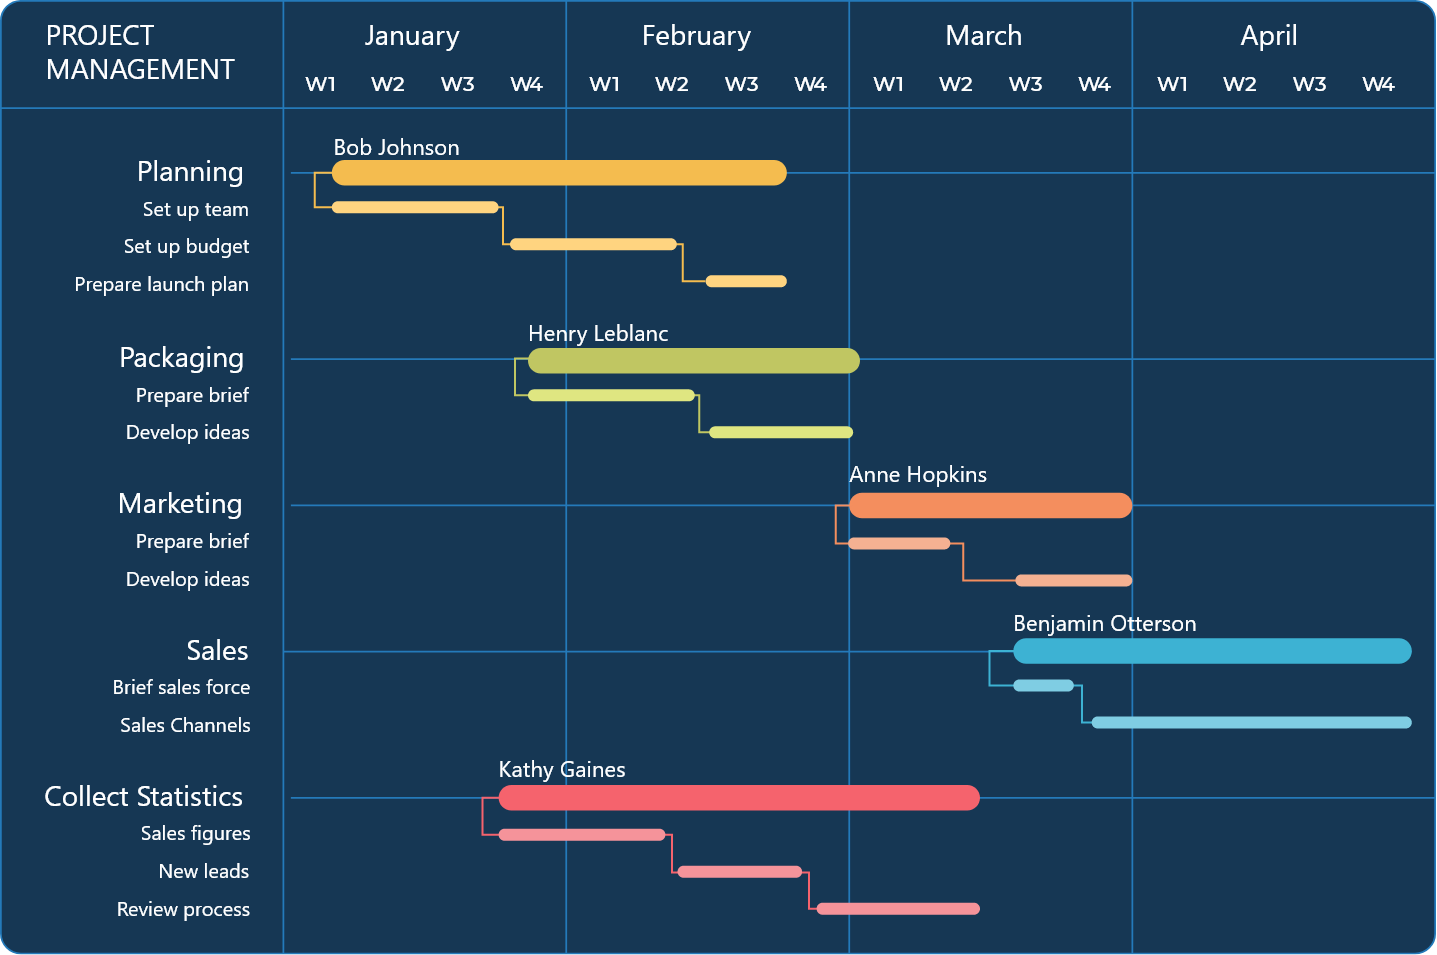
\includegraphics[width=\textwidth]{pictures/упр_диаграма.png}
    \caption{Примерна GANTT диаграма с фази, подзадачи и отговорни лица}
\end{figure}

\subsection{Примерна схема на жизнен цикъл и контролни точки}

\begin{center}
\resizebox{\textwidth}{!}{
\begin{tikzpicture}[
    node distance=1.8cm,
    every node/.style={font=\small},
    phase/.style={
        rectangle,
        draw=black,
        rounded corners,
        minimum width=2.2cm,
        minimum height=0.9cm,
        align=center
    },
    arrow/.style={-{Latex[length=2.5mm]}, thick}
]

\node[phase] (init) {Иницииране};
\node[phase, right=of init] (plan) {Планиране};
\node[phase, right=of plan] (exec) {Изпълнение};
\node[phase, right=of exec] (control) {Контрол};
\node[phase, right=of control] (close) {Приключване};

\draw[arrow] (init) -- (plan);
\draw[arrow] (plan) -- (exec);
\draw[arrow] (exec) -- (control);
\draw[arrow] (control) -- (close);

\draw[arrow, dashed, bend left=25]
(control.south) to (plan.south);

\node[below=0.5cm of init] {M1};
\node[below=0.5cm of plan] {M2};
\node[below=0.5cm of exec] {M3};
\node[below=0.5cm of control] {M4};
\node[below=0.5cm of close] {M5};

\end{tikzpicture}
}
\end{center}

Диаграмата представя основните етапи от жизнения цикъл на проекта и съответните контролни точки (milestones), използвани за проследяване и контрол на напредъка.

\section{Заключение}

Планирането на проекта е фундаментален процес в управлението на проекти, който определя структурата, сроковете, ресурсите и начина на контрол на проектната дейност. Чрез правилно дефиниране на обхвата, изграждане на WBS структура, планиране на ресурси и бюджет, както и използване на методи като CPM, PERT и GANTT диаграми, се осигурява ефективно управление и успешно реализиране на проекта.

Добре изготвеният план-график позволява оптимално разпределение на ресурсите, навременен контрол и минимизиране на рисковете, което е ключово условие за успешното завършване на всеки проект.

\end{FlushLeft}

\end{document}
